\begin{center}
    \fbox{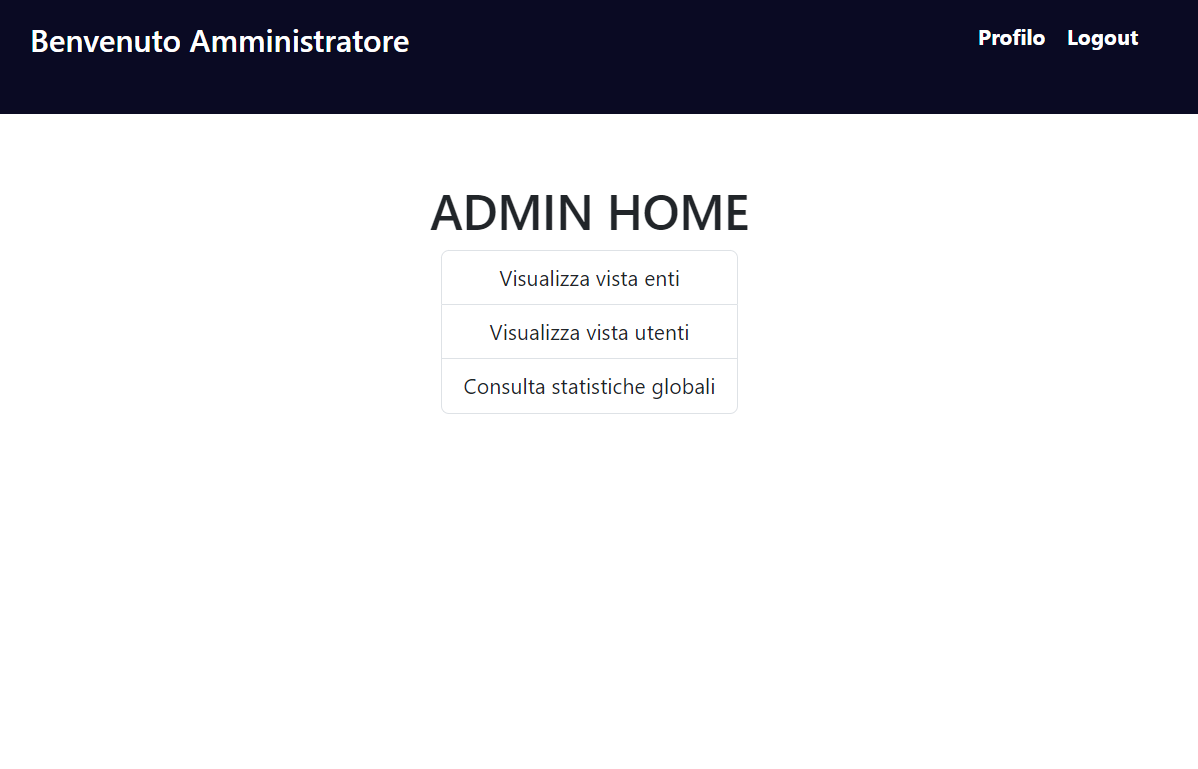
\includegraphics[width=0.95\columnwidth]{amministratore_home.png}}
\end{center}
Una volta effettuato l'accesso l'applicativo offre all'amministratore le seguenti possibilità:
\begin{itemize}
    \item Visualizzare gli enti
    \item Visualizzare gli utenti
    \item Consultazione delle statistiche
\end{itemize}
\begin{center}
    \fbox{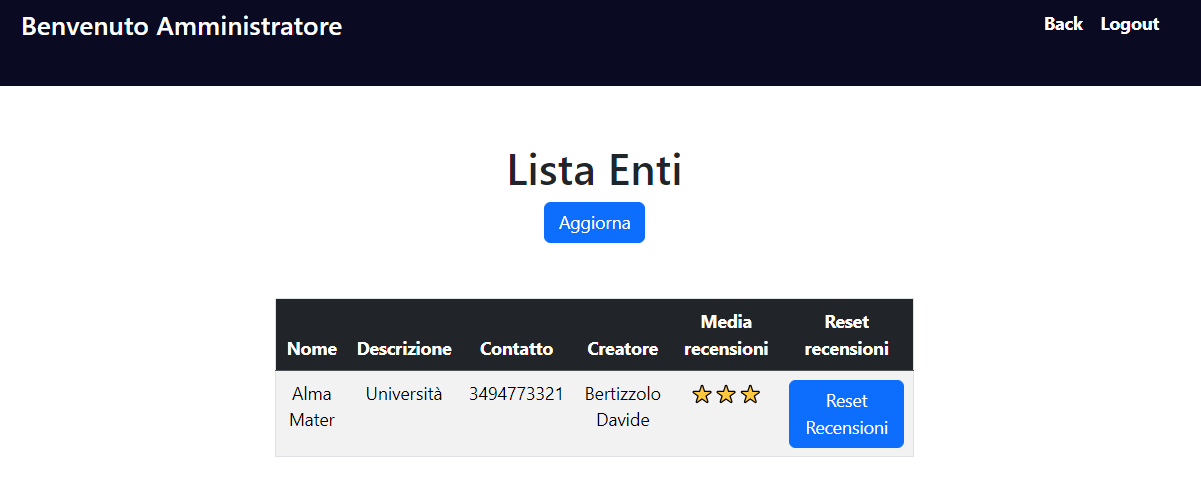
\includegraphics[width=0.95\columnwidth]{amministratore_enti.png}}
\end{center}
Il tasto "Visualizza gli enti" permette di poter visionare l'elenco degli enti registrati all'interno della piattaforma con le relative informazioni e al tasto per resettarne le recensioni, sarà presente un tasto aggiorna in cui si avrà accesso alla lista più recente delle aziende partner.
\begin{center}
    \fbox{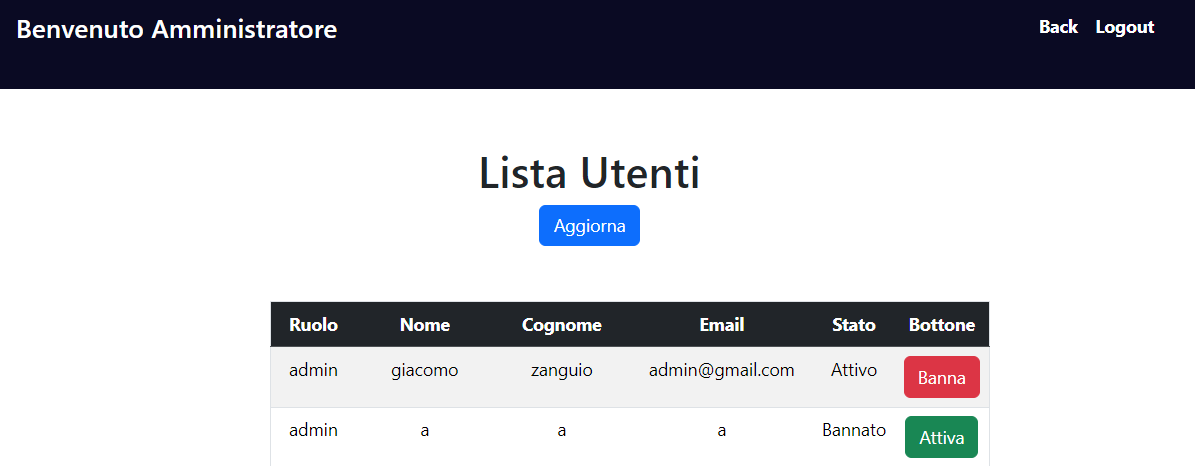
\includegraphics[width=0.95\columnwidth]{amministratore_utenti.png}}
\end{center}
La funzione sarà analoga anche per la lista degli utenti registrati, sarà inoltre possibile interdire l'accesso al sito tramite il tasto "Banna". Una volta bannato l'utente non potrà più effettuare il login. Se l'utente è bannato il tasto cambierà e potra essere riattivato.
\begin{center}
    \fbox{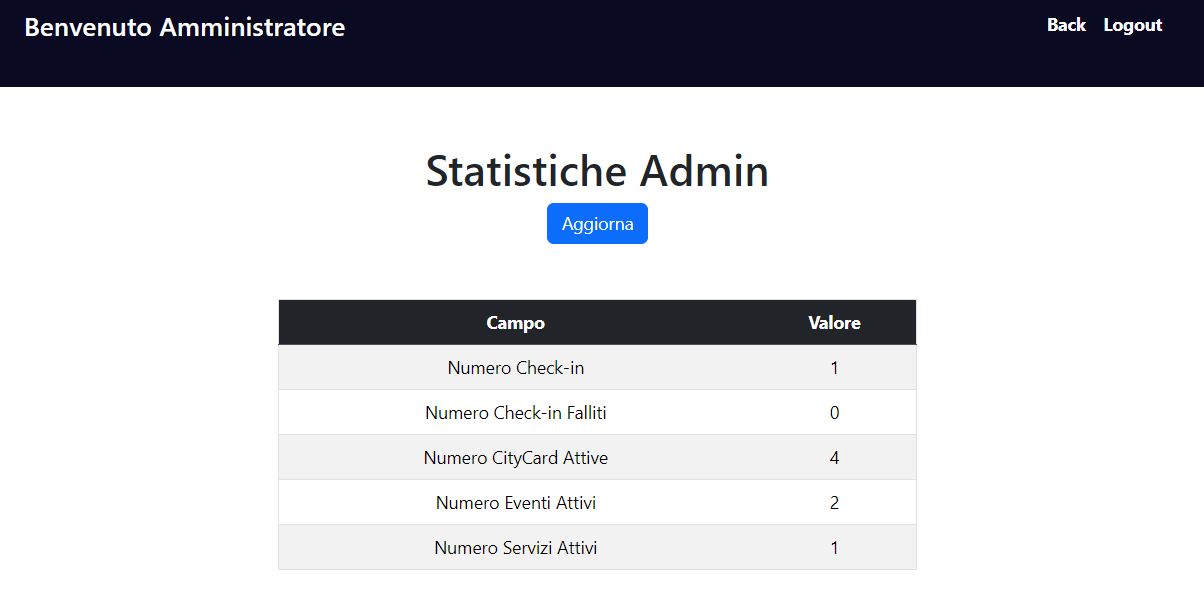
\includegraphics[width=0.95\columnwidth]{amministratore_statistiche.png}}
\end{center}
L'amministratore ha accesso ad alcune statistiche globali della piattaforma.